\PassOptionsToPackage{table}{xcolor}
\documentclass[12pt,letterpaper,twocolumn,openany,nodeprecatedcode,bg=none]{dndbook}
\usepackage[english]{babel}
\usepackage[utf8]{inputenc}
\usepackage{longtable,booktabs,array}
\usepackage{calc}
\usepackage{etoolbox}
\usepackage{caption}
\usepackage{float}
\usepackage{graphicx}
\usepackage{needspace}
\usepackage{tikz}

% Reset zebra striping at the start of every table
\AtBeginEnvironment{longtable}{\rowcolors{1}{white}{gray!10}\small}
\AtBeginEnvironment{table}{\rowcolors{1}{white}{gray!10}}

\providecommand{\pandocbounded}[1]{#1}
\providecommand{\tightlist}{%
  \setlength{\itemsep}{0pt}\setlength{\parskip}{0pt}}

\captionsetup{labelformat=empty}
\setcounter{secnumdepth}{0}
\setlength{\parindent}{0pt}
\setlength{\parskip}{0.5\baselineskip}
\setlength{\headheight}{15pt}

% Prevent orphaned subsections
\let\oldsubsection\subsection
\renewcommand{\subsection}[1]{%
  \needspace{5\baselineskip}%
  \oldsubsection{#1}%
}

\begin{document}
\onecolumn

      \title{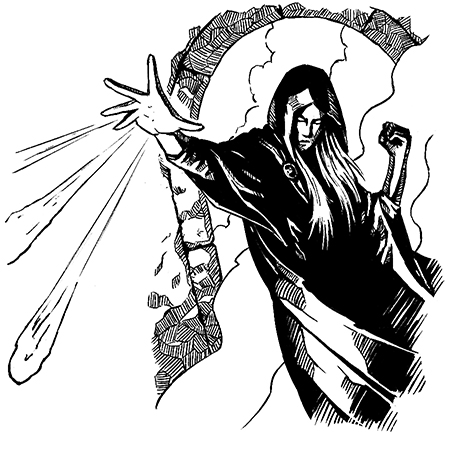
\includegraphics[width=0.9\textwidth,height=0.55\textheight,keepaspectratio]{magicMissile.jpg}\\[1.5cm]Sorcerer}
  \author{Class Handbook}
\date{}
\maketitle

\clearpage
\thispagestyle{empty}
\null\vfill
\begin{center}{\Large\itshape Your trusty class handbook for fantasy
gaming.}\end{center}
\vfill

\clearpage
\thispagestyle{empty}
\begin{center}
\vspace*{\fill}
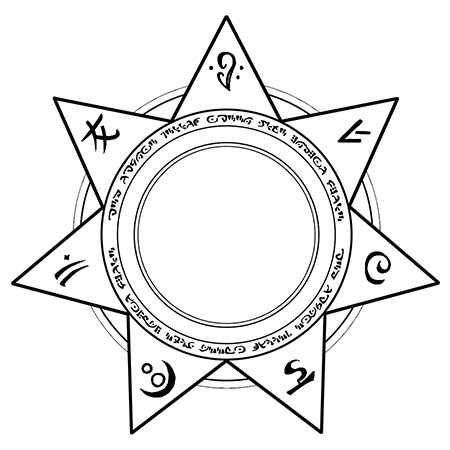
\includegraphics[width=\textwidth,height=0.85\textheight,keepaspectratio]{spellRune.jpg}\par
\vspace{0.4cm}
{\itshape The raw elements of magic are the building blocks of
sorcery.}\par
\vspace*{\fill}
\end{center}

\clearpage
\twocolumn

\section{Sorcerer}\label{sorcerer}

\subsection{Core Sorcerer Traits}\label{core-sorcerer-traits}

\needspace{11\baselineskip}

{\def\LTcaptype{none} % do not increment counter
\begin{table}[!htbp]
\centering
\begin{tabular}{@{}
  >{\raggedright\arraybackslash}p{(\linewidth - 2\tabcolsep) * \real{0.4062}}
  >{\raggedright\arraybackslash}p{(\linewidth - 2\tabcolsep) * \real{0.5938}}@{}}
\toprule\noalign{}
\begin{minipage}[b]{\linewidth}\raggedright
\textbf{Primary Ability}
\end{minipage} & \begin{minipage}[b]{\linewidth}\raggedright
Wisdom
\end{minipage} \\
\midrule\noalign{}
\textbf{Hit Points} & 1d6 \\
\textbf{Saving Throw Proficiencies} & Wisdom, Charisma \\
\textbf{Skill Proficiencies} & Choose 2 skills \\
\textbf{Weapon Proficiencies} & Choose 1 category \\
\textbf{Starting Equipment} & Padded Jacket, Sabre, Dagger, Grimoire \\
\bottomrule\noalign{}
\end{tabular}
\end{table}
}

\subsection{Sorcerer Features}\label{sorcerer-features}

\needspace{20\baselineskip}

{\def\LTcaptype{none} % do not increment counter
\begin{table}[!htbp]
\centering
\begin{tabular}{@{}
  >{\raggedright\arraybackslash}p{(\linewidth - 6\tabcolsep) * \real{0.1020}}
  >{\raggedright\arraybackslash}p{(\linewidth - 6\tabcolsep) * \real{0.2245}}
  >{\raggedright\arraybackslash}p{(\linewidth - 6\tabcolsep) * \real{0.0816}}
  >{\raggedright\arraybackslash}p{(\linewidth - 6\tabcolsep) * \real{0.5918}}@{}}
\toprule\noalign{}
\begin{minipage}[b]{\linewidth}\raggedright
Level
\end{minipage} & \begin{minipage}[b]{\linewidth}\raggedright
Proficiency
\end{minipage} & \begin{minipage}[b]{\linewidth}\raggedright
Mana
\end{minipage} & \begin{minipage}[b]{\linewidth}\raggedright
Class Features
\end{minipage} \\
\midrule\noalign{}
1 & +2 & 2 & Sorcery, Sorcerous Specialty \\
2 & +2 & 3 & --- \\
3 & +2 & 4 & Ability Bonus, Elemental Rune \\
4 & +2 & 5 & --- \\
5 & +2 & 6 & Elemental Resistance \\
6 & +2 & 7 & --- \\
7 & +2 & 8 & Ability Bonus \\
8 & +2 & 9 & --- \\
9 & +3 & 10 & --- \\
10 & +3 & 12 & --- \\
\bottomrule\noalign{}
\end{tabular}
\end{table}
}

\subsection{Level 1: Sorcery}\label{level-1-sorcery}

You channel raw elemental power. Wisdom is your spellcasting ability for
sorcerer features. Your spell attack bonus is your Wisdom modifier +
proficiency bonus. Your spell save DC is 8 + your Wisdom modifier + your
proficiency bonus.

\textbf{Mana Points.} Your magic is powered by mana, as shown in the
Sorcerer Features table. You can spend a number of mana points equal to
your proficiency bonus on any single turn. You regain up to 3 mana
points when you finish a short rest, and all expended mana points when
you finish a long rest.

\textbf{Arcane Bolt.} As an action, make a ranged attack against a
target within 120 feet. On a hit, the target takes 1d10 + your Wisdom
modifier damage. The damage type is fire, cold, or lightning, matching
your Sorcerous Specialty.

Before rolling the attack, you can spend 1 or more mana points to
increase the damage by 1d10 per point spent. If you spend at least 1
mana point, the target takes half damage on a miss.

At 9th level, the base damage increases to 2d10.

\subsection{Level 1: Sorcerous
Specialty}\label{level-1-sorcerous-specialty}

Choose Pyromancy, Cryomancy, or Electromancy. You gain abilities based
on this choice, detailed at the end of this class description. You gain
more abilities from your specialty as you gain levels.

\subsection{Level 3: Ability Bonus}\label{level-3-ability-bonus}

You gain a +1 bonus to two abilities of your choice.

\subsection{Level 3: Elemental Rune}\label{level-3-elemental-rune}

As an action, you can spend 1 or more mana points and store your raw
elemental power in a magical glyph that you place on a surface within 10
feet. The rune is invisible to others but appears to you as a circle of
arcane symbols in a circle occupying a 5 foot diameter. When a creature
steps on the rune, it detonates, dealing 3d6 damage per mana point spent
on this effect.

The damage type is determined by your specialty, either fire, cold,
lightning.

\subsection{Level 5: Elemental
Resistance}\label{level-5-elemental-resistance}

You gain resistance to fire, cold, or lightning damage in accordance
with your sorcery.

\subsection{Level 7: Ability Bonus}\label{level-7-ability-bonus}

You gain a +1 bonus to two abilities of your choice.

\subsection{Level 9: Specialty Bonus}\label{level-9-specialty-bonus}

Your specialty grants you additional features.

\clearpage

\section{Sorcerous Specialty}\label{sorcerous-specialty}

\subsection{Pyromancy}\label{pyromancy}

You are trained in the ways of magical fire. Fire is wild, ambitious,
and alive.

\subsubsection{Level 1: Burning Flames}\label{level-1-burning-flames}

Whenever you roll fire damage, if any die shows its maximum result, roll
an additional die of that type and add it to the damage. Repeat this for
each additional maximum roll.

\subsubsection{Level 1: Flickering
Flame}\label{level-1-flickering-flame}

As an action, you can cause fire to erupt from one of your hands. This
fire sheds bright light for 20 feet and dim light for an additional 20
feet. When you take this action or as a separate action on a later turn,
you can touch a flammable object in melee range and cause it to ignite.

You can choose to douse your hand on your turn without using an action.

\subsubsection{Level 1: Gout of Flame}\label{level-1-gout-of-flame}

As an action, you can make a ranged attack against up to three targets
within 30 feet. On a hit, this attack does 1d6 + your spellcasting
modifier fire damage. The damage increases to 2d6 at level 9.

You can expend mana points to increase the attacks' damage by 2d6 per
point spent, and a target takes half damage on a miss. Spend these
points before rolling your attacks.

\subsubsection{Level 5: Specialty Feature
Choice}\label{level-5-specialty-feature-choice}

Choose one of the features listed below.

\paragraph{Level 5: Flaming Weapon (Choice
1)}\label{level-5-flaming-weapon-choice-1}

As an action, you can expend a mana point to cause a weapon you are
wielding to become wreathed in flames. For the next 10 minutes, whenever
you attack with the weapon it deals an additional 2d6 + your
spellcasting modifier fire damage. The damage increases to 3d6 at level
9. On the turn that you take this action, you may also attack with the
weapon once without using an action.

\paragraph{Level 5: Cinder Cloud (Choice
2)}\label{level-5-cinder-cloud-choice-2}

As an action, spend 1 or more mana points and choose a point within 90
feet. The area within a 20-foot radius of that point fills with smoke
that heavily obscures it for 1 minute per mana point spent or until you
use this feature again. At the end of each of your turns while this
effect lasts, creatures in the smoke-filled area take 1d6 fire damage
per mana point spent on this effect.

\subsubsection{Level 9: Fire Blast}\label{level-9-fire-blast}

As an action, spend 1 or more mana points and choose a point within 120
feet. Each creature within a 20-foot-radius sphere centered on that
point must make a Dexterity saving throw, taking 3d6 fire damage per
mana point spent on a failed save, or half as much on a success.

Until the end of your next turn, creatures that end their turn in the
targeted area take 2 fire damage per mana point spent on this effect.

\subsubsection{Level 9: Specialty Feature
Choice}\label{level-9-specialty-feature-choice}

Choose one of the features listed below.

\paragraph{Level 9: Immolating Rebuke (Choice
1)}\label{level-9-immolating-rebuke-choice-1}

When a creature hits you with a melee attack, you can expend 1 mana
point and deal 2d6 fire damage to it.

Once you use this feature, you cannot use it again until you finish a
short rest.

\paragraph{Level 9: Fire Flight (Choice
2)}\label{level-9-fire-flight-choice-2}

Your flame mastery lets you propel yourself through the air, gaining a
fly speed of 30 feet.

\clearpage

\subsection{Cryomancy}\label{cryomancy}

You are trained in the ways of magical frost. Frost is patient, quiet,
but inevitable.

\subsubsection{Level 1: Freezing Magic}\label{level-1-freezing-magic}

Whenever you deal cold damage to a creature, you can spend a mana point
to force it to make a Constitution saving throw. On a failure, its speed
is reduced by 30 feet until the end of its next turn.

\subsubsection{Level 1: Icy Touch}\label{level-1-icy-touch}

As an action, you can touch a body of water and freeze a 5-foot cube of
it. You can also touch a non-magical object, such as a door, and freeze
it solid. Opening the door requires a Strength (Athletics) check as an
action. The DC equals your spell save DC. You can unfreeze the target at
any time without using an action.

\subsubsection{Level 1: Ice Shard}\label{level-1-ice-shard}

As an action, you can make a ranged attack against a target within 60
feet. On a hit, this attack does 1d8 + your spellcasting modifier cold
damage and all other creatures within 5 feet of the target must make a
Constitution saving throw, taking 1d8 cold damage on a failure. Both of
these damage rolls increase to 2d8 at level 9.

You can expend mana points to increase both of the attacks' damage rolls
by 1d8 per point spent, and a targets takes half damage on a miss or
successful save. Spend these points before rolling your attacks.

\subsubsection{Level 5: Specialty Feature
Choice}\label{level-5-specialty-feature-choice-1}

Choose one of the features listed below.

\paragraph{Level 5: Frozen Fog (Choice
1)}\label{level-5-frozen-fog-choice-1}

As an action, spend 1 or more mana points and choose a point within 90
feet. The area within a 20-foot radius of that point fills with freezing
mist. The area is heavily obscured and is difficult terrain for 1 minute
per mana point spent or until you use this feature again. At the end of
each of your turns while this effect lasts, creatures in the mist-filled
area take 1d4 cold damage per mana point spent on this effect.

\paragraph{Level 5: Ice Shield (Choice
2)}\label{level-5-ice-shield-choice-2}

Once per turn when you or an ally within 5 feet of you takes damage, you
can spend 2 mana points to surround the target with a barrier of ice and
freezing mist. The target gains resistance to all damage types except
psychic until the end of that turn. That resistance applies to the
damage that triggered the use of this feature.

\subsubsection{Level 9: Cone of Cold}\label{level-9-cone-of-cold}

As an action, spend 1 or more mana points. A 60-foot cone of extreme
frost erupts from you. Each creature in the area must make a
Constitution saving throw, taking 2d8 cold damage per mana point spent
on a failed save, or half as much on a success.

Until the end of your next turn, the targeted area becomes difficult
terrain. Any water in the area is frozen solid.

\subsubsection{Level 9: Specialty Feature
Choice}\label{level-9-specialty-feature-choice-1}

Choose one of the features listed below.

\paragraph{Level 9: Frost Cloak (Choice
1)}\label{level-9-frost-cloak-choice-1}

When a creature hits you with a melee attack, you can expend 1 mana
point and deal 2d6 cold damage to it.

Once you use this feature, you cannot use it again until you finish a
short rest.

\paragraph{Level 9: Frozen Fortitude (Choice
2)}\label{level-9-frozen-fortitude-choice-2}

The frost magic that flows through you fortifies your physical form,
granting you superior durability and strengthened willpower. You gain +1
AC and proficiency with Constitution saving throws.

\clearpage

\subsection{Electromancy}\label{electromancy}

You are trained in the ways of magical lightning. Lightning is fast,
precise, yet unpredictable.

\subsubsection{Level 1: Mage Bane}\label{level-1-mage-bane}

Whenever you deal lightning damage to a creature, you can force it to
make a Constitution saving throw. On a failure, it falls prone
immediately.

\subsubsection{Level 1: Static Charge}\label{level-1-static-charge}

As an action, you can spend a mana point to suffuse one creature with
static energy, allowing it to defy gravity for 10 minutes. The effects
are the same as the levitate spell, copied here for reference.

\textbf{Levitate.} One creature or loose object of your choice within
range rises vertically up to 20 feet and remains suspended there. This
can levitate an object that weighs up to 500 pounds. An unwilling
creature that succeeds on a Constitution saving throw is unaffected.

The target can move only by pushing or pulling against a fixed object or
surface within reach (such as a wall or a ceiling), which allows it to
move as if it were climbing. You can change the target's altitude by up
to 20 feet in either direction on your turn. If you are the target, you
can move up or down as part of your move. Otherwise, you can take an
action to move the target, which must remain within 60 feet.

When the effect ends, the target floats gently to the ground if it is
still aloft.

\subsubsection{Level 1: Chain Lightning}\label{level-1-chain-lightning}

As an action, you can make a ranged attack against up to three targets
within 60 feet. On a hit, this attack does 1d6 + your spellcasting
modifier lightning damage. The damage increases to 2d6 at level 9.

You can expend mana points to increase the attacks' damage by 2d6 per
point spent, and a target takes half damage on a miss. Spend these
points before rolling your attacks.

\subsubsection{Level 5: Lightning Whip}\label{level-5-lightning-whip}

As an action, you can expend a mana point to make a melee attack against
a creature within 30 feet using a conjured whip made of pure lightning.
On a hit, this attack does 2d6 + your spellcasting modifier lightning
damage and you can move the target 10 feet in any direction if they are
size Medium or smaller.

At level 9, the damage increases to 4d6 and the whip can move Large
targets.

\subsubsection{Level 5: Specialty Feature
Choice}\label{level-5-specialty-feature-choice-2}

Choose one of the features listed below.

\paragraph{Level 5: Thunder Blast (Choice
1)}\label{level-5-thunder-blast-choice-1}

As an action, spend 1 or more mana points and choose a point within 60
feet. The air at that point erupts with a thunderous blast. Each
creature within a 10-foot radius of that point must make a Constitution
saving throw, taking 1d8 thunder damage per mana point spent on a failed
save, or half as much on a success.

Creatures made of inorganic material such as stone, crystal, or metal
have disadvantage on this saving throw. Non-magical objects
automatically take maximum damage. If you touch the non-magical object,
it takes double damage.

\paragraph{Level 5: Thunderstep (Choice
2)}\label{level-5-thunderstep-choice-2}

Once on your turn, you can spend 2 mana points and cause a burst of
thunder to erupt from under you, allowing you to move up to 30 feet in
any direction without provoking opportunity attacks. This does not
expend an action or any movement.

\subsubsection{Level 9: Lightning Bolt}\label{level-9-lightning-bolt}

As an action, spend 1 or more mana points. A stroke of lightning forms a
line 100 feet long and 5 feet wide blasting out from you in a direction
you choose. Each creature in the line must make a Dexterity saving
throw, taking 3d6 lightning damage per mana point spent on a failed
save, or half as much on a success.

Until the end of your next turn, creatures that failed their saving
throw are dazed.

\subsubsection{Level 9: Specialty Feature
Choice}\label{level-9-specialty-feature-choice-2}

Choose one of the features listed below.

\paragraph{Level 9: Deft Lightning (Choice
1)}\label{level-9-deft-lightning-choice-1}

You learn to deftly weave your lightning around your allies. When you
use magic that deals lightning damage, you may reduce the damage it does
to creatures of your choice to 0.

\paragraph{Level 9: Storm Cloak (Choice
2)}\label{level-9-storm-cloak-choice-2}

When a creature hits you with a melee attack, you can expend 1 mana
point and deal 2d6 lightning damage to it.

Once you use this feature, you cannot use it again until you finish a
short rest.

\paragraph{Level 9: Storm Flight (Choice
3)}\label{level-9-storm-flight-choice-3}

Your lightning mastery lets you defy gravity, gaining a fly speed of 30
feet.

\onecolumn

\clearpage
\thispagestyle{empty}
\begin{center}
\vspace*{\fill}
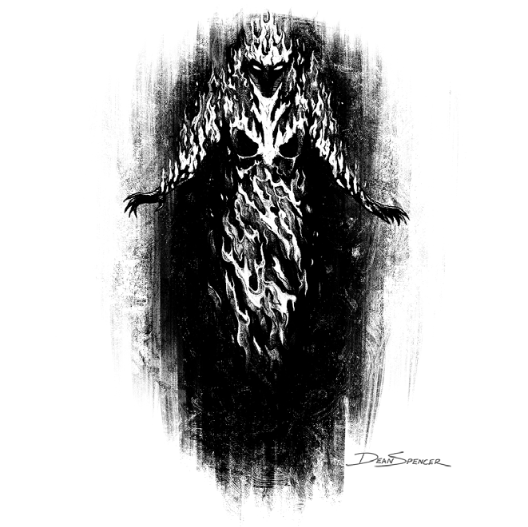
\includegraphics[width=0.7\textwidth,keepaspectratio]{flameAtronach.png}\par
\vspace{0.4cm}
{\itshape Pyromancy is the oldest form of sorcery.}\par
\vspace*{\fill}
\end{center}

\end{document}